\chapter{Methodology} \label{chap:methodology}

\section{Spectral Method}
Spectral method is one of the best tool to solve PDE and ODE problems. \cite{trefethen_spectral_nodate}. The central idea of spectral method is by discretizing the equation, we can transform that to a linear system or an eigenvalue problem.
\subsection{Finite Difference}
Consider equally spaced nodes on domain $[-1,1]$, $\{x_1, x_2, \dots, x_N\}$ with $x_{j+1}-x_{j} = h$ for each $j$, and the set of corresponding function values, $\{ f_1, f_2, \dots, f_N \}$. We can approximate the derivatives using second-order central difference formulas
\[ 
\pdv{f}{z} = \frac{f_{j+1} - f_{j-1}}{2h}
\qquad
\pdv[2]{f}{z} = \frac{f_{j+1} -2f_{j} +f_{j-1}}{h^2}
\]

We can discretize the differentiation operators to the following matrices
\[ 
\pdv{z} \rightarrow D = \frac{1}{2h}\begin{bmatrix}
	0 & 1 & 0 & \dots & 0 \\
	-1 & \ddots & \ddots & \ddots & \vdots \\ 
	0 & \ddots & \ddots & \ddots & 0 \\
	\vdots & \ddots & \ddots & \ddots & 1 \\
	0 & \dots & 0 & -1 & 0 
\end{bmatrix} 
\qquad
\pdv[2]{z} \rightarrow  D^2 = \frac{1}{h^2}\begin{bmatrix}
	-2 & 1 & 0 & \dots & 0 \\
	1 & \ddots & \ddots & \ddots & \vdots \\ 
	0 & \ddots & \ddots & \ddots & 0 \\
	\vdots & \ddots & \ddots & \ddots & 1 \\
	0 & \dots & 0 & 1 & -2 
\end{bmatrix} 
\]

\subsection{Spectral Element}
Suppose the basis functions are $\{u_k(z)\}_{k=1}^\infty$, then the eigenfunction $\tilde{v}$ can be approximated by finite amount of them, $\tilde{v}(z) = \sum_{k=1}^N c_ku_k(z)$ where $c_k$ are coefficients to be determined.

Then by multiplying $u_{i}$ to any term and integrate through the domain, we can discretize the equation. Using the notation of inner product $(f,g)=\int_{-1}^{1} dz fg$, we see that

\[ \int_{-1}^{1} dz \; u_i\tilde{v} = \sum_{j}(u_i,u_j)c_j \]
\[ \int_{-1}^{1} dz \; u_i\pdv{\tilde{v}}{z} = \sum_{j}\left(u_i,\pdv{u_j}{z}\right)c_j \]
\[ \int_{-1}^{1} dz \; u_i\pdv[2]{\tilde{v}}{z} = \sum_{j}\left(u_i,\pdv[2]{u_j}{z}\right)c_j \]

\subsection{Finite Element}
Finite-element method is a generalization of the spectral element method. We are allow to use a set of basis functions similar to spectral method in a cell. The region consists of many of these cells.

The formulation is the same as Eq.(\ref{eq:eigenvalue-problem-SE}). The only difference is that in finite-element we need to solve Eq.(\ref{eq:eigenvalue-problem-SE}) simultaneously for all cells.

\subsection{Spectral Pollution}


\section{Reformulate the Problem for Spectral Method}
Next step we can decouple this equation so that it becomes an eigenvalue problem.
\begin{equation}
	\mqty[ 0 & 1\\ \hat{M} & \hat{N} ]\mqty[ \tilde{v}\\ \omega \tilde{v}] = \omega\mqty[ \tilde{v}\\ \omega \tilde{v}]
	\label{eq:eigenvalue-problem}
\end{equation}
where $O$ is zero matrix, $I$ is identity matrix, and
\begin{align*}
	\hat{M} &= -\left[(1-v_0^2)\pdv[2]{}{z} 
	-\left(3v_0 + \frac{1}{v_0}\right)\pdv{v_0}{z}\pdv{}{z} 
	- \left(1-\frac{1}{v_0^2}\right)\left(\pdv{v_0}{z}\right)^2 
	- \left(v_0+\frac{1}{v_0}\right)\pdv[2]{v_0}{z}\right] \\
	\hat{N} &= -2i\left(v_0\pdv{}{z} +\pdv{v_0}{z} \right) 
\end{align*}
This becomes an algebraic eigenvalue problem if we discretize the operators and the function $\tilde{v}$.




\section{Discretization}

\subsection{Finite Difference}
Using these differentiation matrices, Eq.(\ref{eq:eigenvalue-problem}) becomes
\begin{equation}
	\mqty[ O & I\\ M & N ]\mqty[ \mathbf{\tilde{v}}\\ \omega\mathbf{\tilde{v}} ] = \omega\mqty[ \mathbf{\tilde{v}}\\ \omega\mathbf{\tilde{v}} ]
\end{equation}
where $O$ is a zero matrix, $I$ is an identity matrix, and
\begin{align*}
	M &= -\text{diag}(1-\mathbf{v}_0^2)D^2 
	+\text{diag}\left(3\mathbf{v}_0 + \frac{1}{\mathbf{v}_0}\right) (D\mathbf{v}_0)D 
	+\text{diag}\left(1-\frac{1}{\mathbf{v}_0^2}\right)\left(D\mathbf{v}_0\right)^2 
	+\text{diag}\left(\mathbf{v}_0+\frac{1}{\mathbf{v}_0}\right)(D^2\mathbf{v}_0) \\
	N &= -2i\left(\text{diag}(\mathbf{v}_0)D + D\mathbf{v}_0 \right) 
\end{align*}
Here we abused the notation for the purpose of convenience, $\mathbf{v}_0^2$ means squaring every component of $\mathbf{v}_0$, and $1/\mathbf{v}_0$ denotes 1 divided by all components of $\mathbf{v}_0$.

\subsubsection{Boundary Condition}
We impose Dirichlet boundary condition on the problem, meaning that $\tilde{v}(-1)=\tilde{v}(1)=0$. Further more, the differentiation matrices do not do well on the edges, so during the computation, we remove the first and last row of the differentiation matrices and the vectors $\mathbf{\tilde{v}}$ and $\mathbf{v}_0$. After the computation, we set $\tilde{v}_1=\tilde{v}_N = 0$.


\subsection{Spectral Element}
Suppose the basis functions are $\{u_k(z)\}_{k=1}^\infty$, then the eigenfunction $\tilde{v}$ can be approximated by finite amount of them, $\tilde{v}(z) = \sum_{k=1}^N c_ku_k(z)$ where $c_k$ are coefficients to be determined.

\begin{equation} \label{eq:eigenvalue-problem-SE}
	\mqty[ O & I\\ M & N ]\mqty[ \mathbf{c}\\ \omega\mathbf{c} ] = \omega\mqty[ \mathbf{c}\\ \omega\mathbf{c} ]
\end{equation}
where $O$ is a zero matrix, $I$ is an identity matrix, and
\begin{align*}
	M_{jk} &= -\int_{-1}^{1}dz \; u_{j} \left[(1-v_0^2)\pdv[2]{}{z} 
	-\left(3v_0 + \frac{1}{v_0}\right)\pdv{v_0}{z}\pdv{}{z} 
	- \left(1-\frac{1}{v_0^2}\right)\left(\pdv{v_0}{z}\right)^2 
	- \left(v_0+\frac{1}{v_0}\right)\pdv[2]{v_0}{z}\right] u_{k} \\
	N_{jk} &= -2i\int_{-1}^{1}dz \; u_{j}\left(v_0\pdv{}{z} +\pdv{v_0}{z} \right)u_{k}
\end{align*}

\subsubsection{Boundary Conditions and Basis Function}
To satisfy the Dirichlet boundary condition, $\tilde{v}(\pm 1)=0$, we can choose a set of basis functions that satisfy the boundary condition $u_k(\pm 1)=0,\forall k\in\mathbb{N}$. For example, the sine functions
\[ u_n(z) = \sin(\frac{n\pi}{2}(z+1)), n\in\mathbb{N} \]
is a set of basis functions that satisfy the Dirichlet boundary condition.


\subsection{Finite Element}
Finite-element method is a generalization of the spectral element method. We are allow to use a set of basis functions similar to spectral method in a cell. The region consists of many of these cells.

The formulation is the same as Eq.(\ref{eq:eigenvalue-problem-SE}). The only difference is that in finite-element we need to solve Eq.(\ref{eq:eigenvalue-problem-SE}) simultaneously for all cells.

\subsubsection{Boundary Conditions and B-Spline}
The B-Spline is a commonly used basis function for finite-element method. B-Spline can be defined recursively starting with piecewise constants [reference needed]

\begin{equation}
	B_{i,0}(\xi) = \begin{cases}
		1, &\text{if } \xi_i\leq \xi \leq \xi_{i+1} \\
		0, &\text{otherwise}
	\end{cases}
\end{equation}
For $j\in\mathbb{N}$, they are defined by
\begin{equation}
	B_{i,j}(\xi) = \frac{\xi-\xi_i}{\xi_{i+j}-\xi_i}B_{i,j-1}(\xi) 
	+ \frac{\xi_{i+j+1}-\xi}{\xi_{i+j+1}-\xi_{i+1}}B_{i+1,p-1}(\xi) 
\end{equation}
where $\mathbf{\xi}=[\xi_0,\cdots,\xi_m]$ is called the knot vector, where $m=n+j+1$ where $n+1$ is the number of B-Splines and $j$ is the degree of B-Spline polynomials. The knot vector defines the shapes of the B-Splines, see Fig.\ref{fig:bspline}. The variable $\xi$ is within the range $[\xi_0, \xi_m]$. 

Any function $u(x)$ on $[\xi_0,\xi_N]$ can be approximated by
\[ u(x) \simeq \sum_{j=0}^{n} c_jB_{i,j}(x) \]

The Dirichlet boundary condition can be set by letting the coefficients of the first and last B-Spline to 0, $c_{0}=c_{n} = 0$, where $N$ is the number of B-Splines.


\begin{figure} [H]
	\centering
	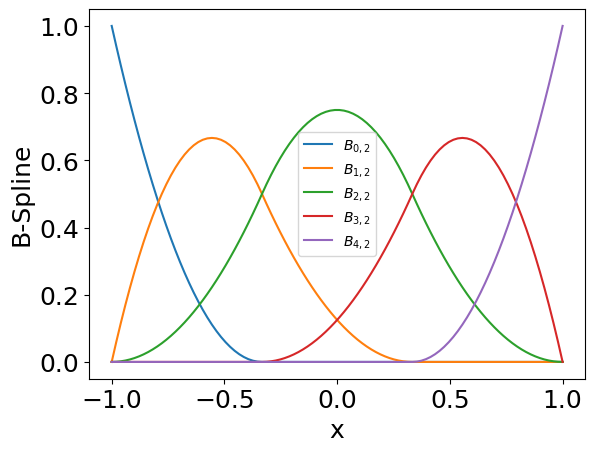
\includegraphics[width=0.7\linewidth]{img/governing-equations/bspline}
	\caption{An example of open uniform quadratic B-Spline on $[-1,1]$. The knot vector is $[-1,-1,-1,-1/3,1/3,1,1,1]$.}
	\label{fig:bspline}
\end{figure}


\section{Shooting Method}
Shooting method can be used to solve eigenvalue problem with specified boundary values,
\begin{equation} \label{eq:boundary-eigenvalue-problem}
g(\tilde{v}(z);\omega) = 0,
\quad
z_l \leq z \leq z_r,
\quad
\tilde{v}(z_l) = \tilde{v}_l, \tilde{v}(z_r) = \tilde{v}_r
\end{equation}
where $\omega$ is the eigenvalue to be solved.

Suppose a eigenvalue problem can be formulated as
\[ \dv{z}\mathbf{u} = \mathbf{f}(\mathbf{u},z;\omega),
\quad
z_l<z<z_r,
\quad
\mathbf{u}(z_l) = \mathbf{u}_l
\]
where $\mathbf{u}\in\mathbb{R}^2$. Fixed an $\omega$, we can approximate $\mathbf{u}(z_r)$ by applying algorithms such as Runge-Kutta or Leap-frog.

Define $F$ by $F(\mathbf{u}_l;\omega)=\tilde{v}(z_r;\omega)$. This function $F$ takes in the initial value $\mathbf{u}_l$ and a fixed $\omega$, and outputs the "landing point" $\tilde{v}(z_r;\omega)$. If $\omega$ is an eigenvalue of Eq.(\ref{eq:boundary-eigenvalue-problem}), then $\tilde{v}(z_r;\omega) = \tilde{v}_r$. Now we can find eigenvalues to Eq.(\ref{eq:boundary-eigenvalue-problem}) by solving the roots to the scalar equation
\[h(\omega) = F(\mathbf{u}_l;\omega) - \tilde{v}_r\]

\subsection{Solve as Root Finding Problem}
Eq.(\ref{eq:polynomial-eigenvalue-problem}) can be rewrite as 
\begin{align*}
v' &= u\\
u' &= \frac{-1}{1-v_0^2}\left[
    \omega^2v + 2i\omega(v_0+v_0'v) - \left(3v_0 - \frac{1}{v_0}\right)v_0'u - \left(1-\frac{1}{v_0}^2\right)(v_0')^2v - \left(v_0+\frac{1}{v_0}v_0'' v\right)
\right]
\end{align*}
and $v(0)=c_0=1,u(0)=c_1=(2i\omega v_0'-2v_0'')/2v_0'$. Moreover, $u'(0)=c_2=-((v_0')^4+(2i\omega v_0' + (v_0')^2 - v_0'')(i\omega v_0' - v_0''))/(v_0'(2i\omega-6v_0'))$
\subsection{Expansion at Singularity}
If the equilibrium velocity profile $v_0$ is a transonic profile, then $v_0(0) = 1$ at the throat of the magnetic mirror configuration. This is a singularity. More specifically, it is a regular singular point. 

In order to supply initial values to shooting method, we need to expand Eq.(\ref{eq:polynomial-eigenvalue-problem}) at the singularity.

Since 
\begin{equation}
   \begin{aligned}
    1-v_0^2 &= -2v_0'(0)z\\
    3v_0 + \frac{1}{v_0} &= 4 - 2v_0'(0)z \\
    1-\frac{1}{v_0^2} &= 2v_0'(0)z \\
    v_0 + \frac{1}{v_0} &= 2
   \end{aligned} 
\end{equation}

Then Eq.(\ref{eq:polynomial-eigenvalue-problem}) becomes
\begin{equation}
    \begin{aligned}
        -& 2v_0'(0)z\pdv[2]{\tilde{v}}{z} \\
        +& [2i\omega - 4v_0'(0) + (2i\omega + 2v_0'(0))z]\pdv{\tilde{v}}{z} \\
        +& (2i\omega v_0'(0) - 2v_0''(0) - 2v_0'(0)^3z)\tilde{v}
        = 0
    \end{aligned}
    \label{eq:perturbed-equation-full}
\end{equation}

Since we are expanding at $z=0$, we drop all $z$ terms except the first term (second-order derivative term).

\[ - 2v_0'(0)z\pdv[2]{\tilde{v}}{z}
+ (2i\omega - 4v_0'(0))\pdv{\tilde{v}}{z} 
+ (2i\omega v_0'(0) - 2v_0''(0))\tilde{v}
= 0 \]

Dividing by the first coefficient, we have
\begin{equation}
    z\pdv[2]{\tilde{v}}{z} + a\pdv{\tilde{v}}{z} + b\tilde{v} = 0
    \label{eq:perturbed-equation}
\end{equation}
where
\[ a = \frac{2i\omega - 4v_0'(0)}{-2v_0'(0)} = 2 - \frac{i\omega}{v_0'(0)}; \quad 
b = \frac{2i\omega v_0'(0) - 2v_0''(0)}{-2v_0'(0)} = \frac{v_0''(0)}{v_0'(0)} -i\omega
\]

Use Frobenius method, we assume $\tilde{v} = \sum_{n\geq 0}c_nz^{n+r}$, plug Eq.(\ref{eq:perturbed-equation}) we have
\[ \sum_{n \geq 0} (n+r)(n+r+1) c_n z^{n+r-1} + a(n+r)c_nz^{n+r-1} + bc_nz^{n+r} = 0\]
Shift the power of the last term we get
\[ \sum_{n \geq 0} (n+r)(n+r+1) c_n z^{n+r-1} + a(n+r)c_nz^{n+r-1} + \sum_{n \geq 1} bc_{n-1}z^{n+r-1} = 0\]

Setting $n=0$, we get the indicial equation
\[ c_0 r(r-1) + c_0 ar = 0 \Rightarrow c_0r(r+a-1) = 0 \]
We get two different roots, $r=0$ and $r=1-a$. They correspond to finite solution and diverging solution near the singularity, respectively.

The coefficients are given by reccurence relation
\[ (n+r)(n+r-1)c_n + a(n+r)c_n + bc_{n-1} = 0 
\Rightarrow
c_n = \frac{-bc_{n-1}}{(n+r)(n+r-1+a)}
\]
Solving this relation we get explicit expression for $c_n$,
\begin{equation}
    \begin{aligned}    
        c_n &= \frac{(-1)^n b^n c_0}{\prod_{k=0}^{n-1} (n+r-k)(n+r-1+a-k)} \\
        &= (-1)^n b^n c_0 \frac{\Gamma(r+1)\Gamma(r+a)}{\Gamma(n+r+1)\Gamma(n+r+a)}
    \end{aligned}
    \label{eq:coefficient}
\end{equation}

\begin{itemize}
    \item Worth to mention that the diverging solution goes like 
    \[ \tilde{v}(z) \sim z^{1-a} = z^{-1-\omega_i/v_0'(0)}z^{i\omega_r/v_0'(0)}  \]
    where $\omega = \omega_r + i\omega_i$. Meaning that the solution will be divergent iff $\omega_i > -v'(0)$.
    \item Droping the $z$ terms in Eq.(\ref{eq:perturbed-equation-full}) has no effect on the first order correction ($\tilde{v}$ is the same up to $z$ term).
\end{itemize}
